\section{Controlled Empirical Testbed and Attributional Protocol}
\label{sec:methodology}

This section details the operational wind farm testbed, the five-dimensional constraint lifecycle taxonomy, and our Controlled Attribution Protocol designed to distinguish genuine domain physical guidance from confounding alternative mechanisms.

\subsection{The Five-Dimensional Constraint Lifecycle Taxonomy}
Designating a neural forecaster as ``physics-constrained'' often groups fundamentally disparate mathematical, architectural, and data-flow operations under a single heading \cite{lipton2019}. To establish an operational foundation for systematic auditing and controlled benchmarking, we define a structured \textbf{Constraint Lifecycle Taxonomy}.

The primary unit of analysis is the individual forecasting model, characterized by its operational constraint mechanism. Formally, we characterize the primary constraint architecture $C$ as a 5-tuple operating across orthogonal lifecycle stages:
\begin{equation}
C = \big\langle \mathcal{D}_1, \mathcal{D}_2, \mathcal{D}_3, \mathcal{D}_4, \mathcal{D}_5 \big\rangle,
\label{eq:constraint_tuple}
\end{equation}
where $\mathcal{D}_1$ represents parameter provenance, $\mathcal{D}_2$ denotes application stage, $\mathcal{D}_3$ specifies inference telemetry requirements, $\mathcal{D}_4$ captures implementation software fidelity, and $\mathcal{D}_5$ assesses evaluation validity and harm reporting (Figure~\ref{fig:lifecycle}).

\begin{figure*}[!t]
\centering
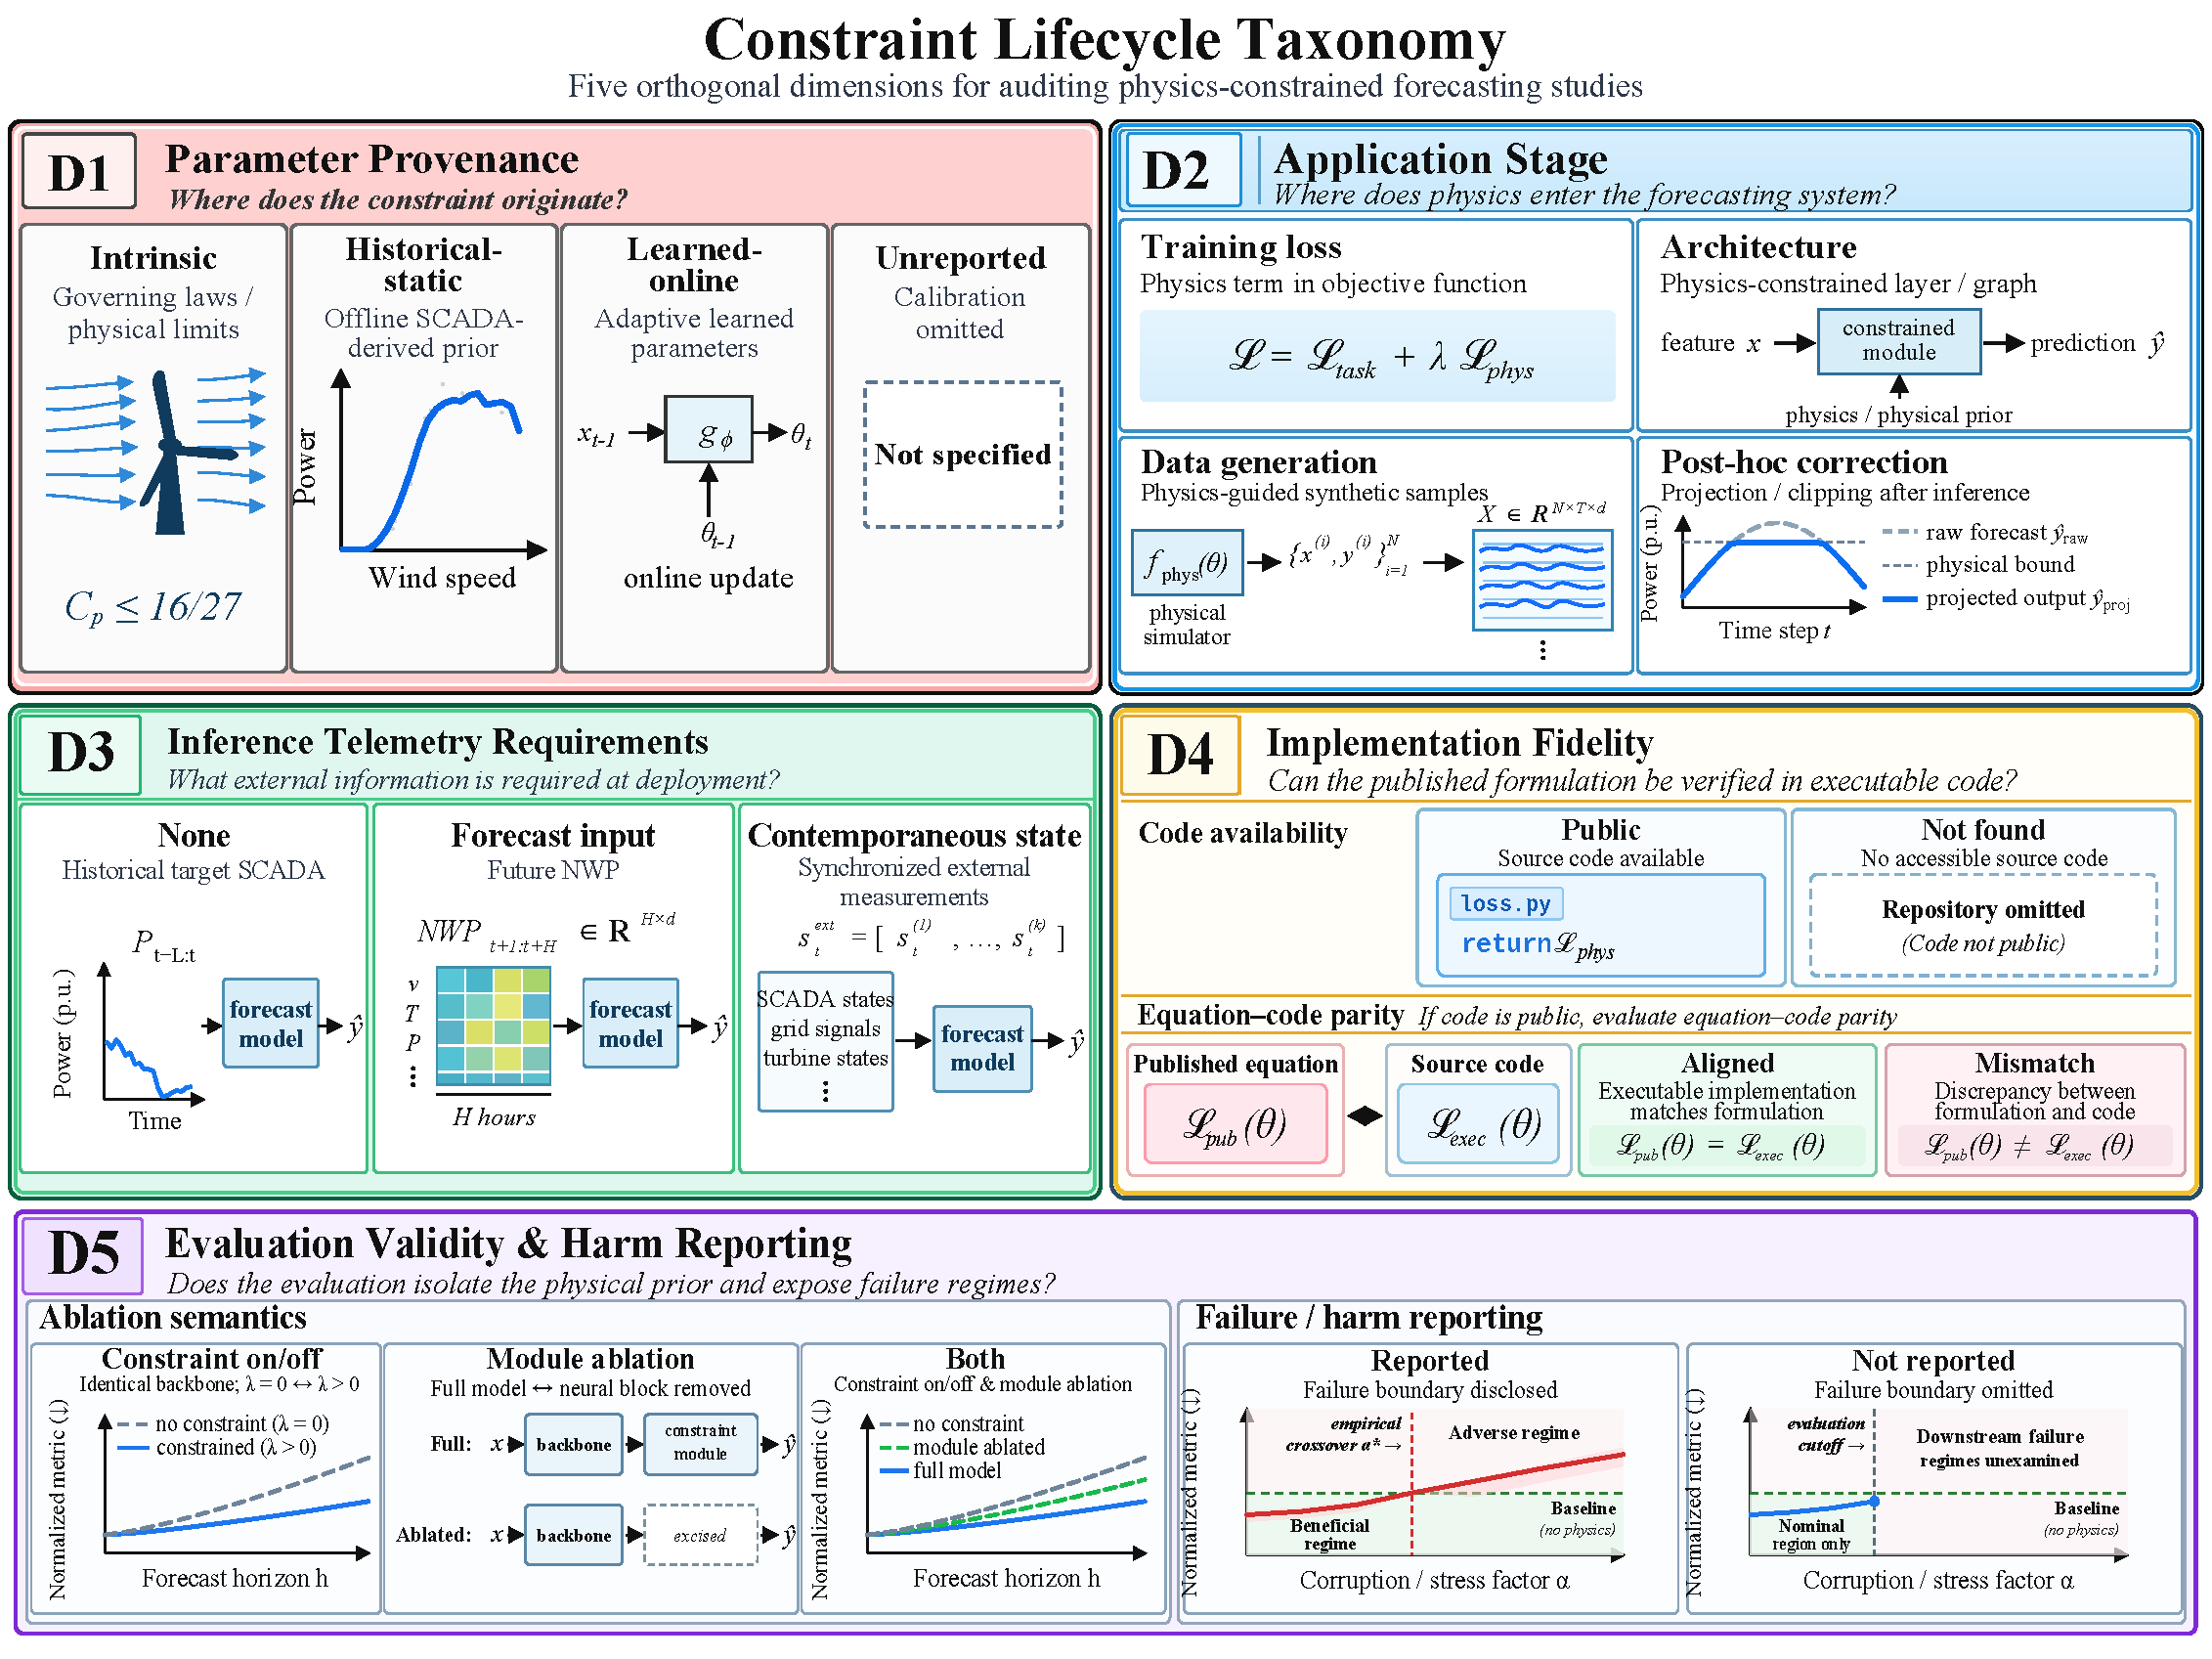
\includegraphics[width=\textwidth]{fig_constraint_lifecycle.pdf}
\caption{The Five-Dimensional Constraint Lifecycle Framework. Tracking domain physical constraints from parameter origin ($\mathcal{D}_1$) through computational graph formulation ($\mathcal{D}_2$), operational telemetry dependency ($\mathcal{D}_3$), software implementation parity ($\mathcal{D}_4$), and evaluation validity and harm reporting ($\mathcal{D}_5$).}
\label{fig:lifecycle}
\end{figure*}

\paragraph{Dimension 1: Parameter Provenance ($\mathcal{D}_1$)}
Identifies the calibration origin of constraint parameters: (1)~\textit{intrinsic}, where parameters derive analytically from physical invariants without empirical fitting (e.g., Betz limit $C_p \le 16/27$ or kinematic wake equations); (2)~\textit{historical-static priors}, where reference power curves or joint probability distributions are estimated offline on historical SCADA archives and held static during deployment; (3)~\textit{learned-online}, where parameters adapt dynamically via auxiliary neural subnetworks; and (4)~\textit{unreported}, where calibration details are omitted.

\paragraph{Dimension 2: Application Stage ($\mathcal{D}_2$)}
Identifies where domain physics enters the computational pipeline: (1)~\textit{training-loss regularization} ($\mathcal{L} = \mathcal{L}_{\text{task}} + \lambda \mathcal{L}_{\text{phys}}$); (2)~\textit{inference-architecture constraints}, modifying layers to project outputs onto admissible manifolds; (3)~\textit{data-generation priors}, synthesizing augmented training scenarios; and (4)~\textit{post-hoc correction filters}, applied externally after inference.

\paragraph{Dimension 3: Inference Telemetry Requirements ($\mathcal{D}_3$)}
Identifies external operational data streams required during real-time deployment: (1)~\textit{none}, relying solely on target turbine historical power; (2)~\textit{forecast-input}, requiring future numerical weather prediction (NWP) inputs; and (3)~\textit{contemporaneous-state}, requiring synchronized real-time measurements from adjacent turbines or met masts.

\paragraph{Dimension 4: Implementation Fidelity ($\mathcal{D}_4$)}
Evaluates whether public software faithfully executes published mathematical formulations: (1)~\textit{code-aligned}, where public source code strictly matches published equations; (2)~\textit{code-mismatch}, where the codebase exhibits an algebraic or directional deviation; and (3)~\textit{not-found}, where no public repository or script accompanies the study.

\paragraph{Dimension 5: Evaluation Validity and Harm Reporting ($\mathcal{D}_5$)}
This dimension contains two complementary subfields: (i)~\textit{ablation semantics}, classified as \textit{constraint-on-off} (where treatment and baseline share identical parameter capacity, differing only in the activation of the physical prior, $\lambda=0$ vs.\ $\lambda>0$), \textit{module-ablation} (where the ablation excises an entire multi-parameter neural block), or \textit{both}; and (ii)~\textit{harm reporting}, classified as \textit{reported} (explicitly documenting operating regimes or failure boundaries where physical constraints degrade downstream performance) or \textit{not-reported}.

\subsection{Multi-Site Operational Wind Farm Testbed and SCADA Telemetry}
To ground the empirical benchmark in real-world power system operations across diverse terrains, we established an operational testbed across three commercial UK wind farms with 10-minute SCADA telemetry:
\begin{itemize}[leftmargin=*]
\item \textbf{Kelmarsh Wind Farm} (Northamptonshire, England): Located in flat open agricultural terrain, comprising six Senvion MM92 turbines (rated 2.05~MW each, hub height 78~m, farm capacity 12.3~MW), evaluated over $N_{\text{train}} = 5,098$ clean intervals as our primary development benchmark (8,212 test origins, 49,272 forward delivery steps across full-year 2017) \cite{zenodo_kelmarsh}.
\item \textbf{Hill of Towie Wind Farm} (Drummuir, Scotland): Located in complex upland terrain featuring micro-topographical wake interactions, comprising 21 Siemens SWT-2.3-82 turbines (rated 2.3~MW each, hub height 60~m, farm capacity 48.3~MW), evaluated as an independent spatiotemporal extrapolation benchmark across full-year 2017 with 7,599 forecast origins (45,594 delivery steps) \cite{zenodo_hilloftowie}.
\item \textbf{Penmanshiel Wind Farm} (Scottish Borders): Located in undulating upland terrain, comprising 14 Senvion MM82 turbines (rated 2.05~MW each, farm capacity 28.7~MW), configured with a sample-restricted training partition ($N_{\text{train}} = 1,583$) across 8,440 test origins to evaluate model behavior in this sample-restricted setting \cite{zenodo_penmanshiel}.
\end{itemize}
Standard data sanitation protocols removed periods of turbine curtailment, anemometer icing, and communication dropouts ($P \le 0$ when $v > v_{\text{cut-in}}$ or active power frozen for $>6$ consecutive steps). Real-world balancing price dynamics were evaluated using official 2017 UK Elexon BSC System Buy Prices (mean \pounds 44.27/MWh, peak \pounds 1,509.80/MWh, with 68 negative price periods).

\subsection{The Controlled Attribution Protocol}
To overcome the confounding inherent in standard benchmarking, we establish the \textbf{Controlled Attribution Protocol}. Rather than comparing a physics-constrained neural network against an unrelated data-driven baseline or excising neural submodules, this protocol holds all non-physical factors strictly invariant:
\begin{enumerate}[leftmargin=*]
\item \textbf{Backbone and Parameter Parity}: All candidate models within each benchmark arm share identical neural architectures (DLinear, \cite{zeng2023dlinear}), identical layer counts, and identical parameter weights.
\item \textbf{Data Splits and Optimization Schedules}: Training, validation, and test splits are strictly synchronized across all arms. Within each controlled comparison block, treatment and control arms used identical paired random seeds. Seed sets differed across distinct experiment families and are reported explicitly in the corresponding tables and supplementary experiment registry.
\item \textbf{Form- and Weight-Matched Pseudo-Scrambled Controls}: To separate authentic aerodynamic guidance from non-specific numerical smoothing, we construct negative controls that permute the empirical wind-to-power mapping along the wind speed axis while holding network architectures, loss formulations, and penalty weights $\lambda$ 100\% identical.
\item \textbf{Decoupled Post-Hoc Quantile Calibration}: All forecasters undergo identical post-hoc scalar quantile calibration ($\delta^* = \arg\min_\delta \hat{\mathcal{R}}_{\text{val}}(f_\theta + \delta)$ at $r=2, q=1/3$), evaluated strictly on the 2016 validation year before accessing the 2017 test timeline. This ensures that reported differences reflect genuine representation accuracy rather than uncalibrated quantile offsets.
\end{enumerate}

\subsection{Controlled Ablation Arms and Boundary Stress Tests}
The forecasting suite evaluates an input lookback of $L=36$ (6 hours) and a forecast horizon of $H=36$ (6 hours), with downstream economic dispatch evaluated over the next-hour delivery window $H_{\text{disp}} = \{1, \dots, 6\}$ and an origination stride of $S=6$ steps to prevent overlapping settlement intervals. The experimental arms comprise:
\begin{enumerate}[leftmargin=*]
\item \textit{Unconstrained DLinear}: Baseline linear mapping across trend and seasonal decomposition ($\lambda=0$) \cite{zeng2023dlinear}.
\item \textit{Authentic Empirical Power Curve Prior}: Penalizing squared deviations from site-specific empirical power curves across penalty weights $\lambda \in \{0.01, 0.1, 1.0\}$; during test inference, the model operates purely on historical power telemetry ($\mathcal{D}_3 = \texttt{none}$).
\item \textit{Form- and Weight-Matched Pseudo-Scrambled Prior}: Permuting the aerodynamic power curve mapping across identical $\lambda \in \{0.01, 0.1, 1.0\}$.
\item \textit{Info-Symmetric Reference Arm}: Supplying contemporaneous wind speed directly as an unconstrained input feature to assess whether symmetric error reductions align with operational dispatch risk.
\item \textit{Strictly Budget-Matched Information Ablation} ($N_{\text{prior}}=N_{\text{train}}=500$): To decouple domain prior geometry from historical sample expansion, models trained on restricted windows ($N_{\text{train}}=500$, $\approx 21$ days) are evaluated against both budget-matched priors (fitted strictly on the identical 500 samples) and full-history priors (fitted on 7--10 months).
\item \textit{Within-Site Learning Curves}: Subsampling training volume across $N_{\text{train}} \in \{500, 1000, 1500, 3000, 5000\}$ on Kelmarsh and Hill of Towie across five random seeds.
\item \textit{Continuous Prior Corruption and Engineering Drift}: Continuously interpolating between authentic and scrambled priors ($\alpha \in [0.0, 1.0]$), simulating aerodynamic aging via rated capacity derating (0\% to 20\%), and applying anemometer calibration drift ($-15\%$ to $+15\%$).
\item \textit{Training Proxy Staleness Scan}: Scanning historical wind speed proxy lag $k \in \{6, 12, 18, 36\}$ steps (1h to 6h delay) in the training loss objective.
\item \textit{Cross-Backbone Architectural Probe (PatchTST)}: Evaluating PatchTST (\cite{nie2023patchtst}, patch length 6, stride 4, 2-layer encoder with RevIN) across 60 independently trained models (3 farms $\times$ 4 constraints $\times$ 5 seeds) under nominal regularization ($\lambda=0.01$).
\end{enumerate}

Statistical significance was evaluated via 2,000-replication circular block paired bootstrapping with 7-day block lengths ($L=1,008$ intervals) on full-year continuous telemetry (Kelmarsh and Hill of Towie) to account for meteorological autocorrelation, combined with multi-seed standard deviations to capture optimization variance across the unified five seeds.

\subsection{Governing Attribution Scope: What Is Evaluated vs.\ What Is Not}
\label{subsec:governing_identification}
To ensure that empirical observations are not conflated with broader causal or mechanistic claims, we explicitly define the formal attributional scope of our experimental design:

\paragraph{Empirically Distinguished Under the Controlled Protocol}
\begin{enumerate}[leftmargin=*, label=(\alph*)]
\item \textit{Prior-Specific Inductive Guidance vs.\ Generic Regularization}: Under the tested matched-control protocol, divergence between authentic and pseudo-scrambled priors provides evidence that the observed performance shift is specific to the empirical aerodynamic mapping, rather than being explained by penalty form and weight alone.
\item \textit{Independence from Historical Volume Expansion}: The 500-sample budget-matched control isolates whether empirical benefits persist when prior fitting is restricted strictly to the contemporaneous training window, bounding the influence of historical telemetry volume.
\item \textit{Empirical Operating Boundaries}: Parametric scans map empirical sensitivity to sample size attenuation ($N_{\text{train}} \in \{500, \dots, 5000\}$), continuous prior corruption crossover regions ($\alpha$), aerodynamic derating, and training-loss proxy staleness ($k$) within the tested configurations. These values are empirical crossover locations along the evaluated perturbation grid, not population-level physical thresholds.
\end{enumerate}

\paragraph{Not Formally Identified (Confounding Disclaimers)}
\begin{enumerate}[leftmargin=*, label=(\roman*)]
\item \textit{Abstract Causal Effects of Physics}: Our experiments evaluate specific empirical power-curve and distributional constraints under evaluated configurations; they do not establish universal causal claims for ``physics'' as an abstract treatment across arbitrary architectures or energy systems.
\item \textit{Cross-Site Topographical Causation}: Differences across Kelmarsh, Hill of Towie, and Penmanshiel confound topographic complexity with turbine ratings (2.05\,MW vs.\ 2.30\,MW), hub heights, wake geometry, and local micro-climates; topography remains an observational covariate rather than an isolated treatment.
\item \textit{Direct Bias--Variance Component Estimation}: Our theoretical framework provides a decision-theoretic representation/calibration/cross-coupling decomposition; we do not directly estimate classical statistical bias and variance scalars from empirical data.
\end{enumerate}
